\documentclass{git_course}

\title{Version control with Git}
\author{Paul Cochrane}
\date{\today}

\begin{document}

\maketitle

\begin{frame}
\begin{multicols}{2}
\begin{spacing}{0.8}
\tableofcontents
\end{spacing}
\end{multicols}
\end{frame}


%%%%%%%%%%%%%%%%%%%%%%%%%%%%%%%%%%%%%%%%%%%%%%%%%%%%%%%%%%%%%%%%%%%%%%%%%%%%
\section{About the course}

\begin{frame}
\frametitle{Course goals}

At the end of this course you should:

\begin{itemize}
    \item feel comfortable using Git
    \item know where to get further help, if necessary
    \item be able to use Git on private projects
    \item be able to collaborate with others using remote repositories
\end{itemize}
\end{frame}

\begin{frame}
\frametitle{Course outline}
\begin{itemize}
    \item Introduction to Git and version control systems
    \item Installing Git
    \item Creating a first repository
    \item Getting help
    \item Tracking/staging/committing
    \item Configuring repositories
    \item General workflow
    \item Getting repository information
    \item Working with others
    \item Using branches and tags
    \item Rewriting history
    \item Contributing to Open Source projects
\end{itemize}
\end{frame}

% XXX: course flow as diagram

\begin{frame}
\frametitle{Course information}
\begin{itemize}
    \item Feedback most welcome
    \item Slides and notes are available on the GitHub docs site for the
        course:\\
        {\footnotesize \url{https://paultcochrane.github.io/version\_control\_course/}}
    \item You can submit pull requests, file issues, on GitHub:\\
        {\footnotesize \url{https://github.com/paultcochrane/version\_control\_course/}}
\end{itemize}
\end{frame}

\begin{frame}
\frametitle{About me}
\begin{itemize}
    \item Physicist from New Zealand
    \item Have been involved in scientific computing and development of
        scientific software in Australia and Germany
    \item Led the scientific computing group at the Regional Computing
        Centre for Lower Saxony
    \item Currently a software developer for a startup in Bremen
        specialising in delivery of satellite-based information to users in
        polar regions
    \item Active in the Perl language community
\end{itemize}
\end{frame}

\section{Version control systems and Git history}

\begin{frame}
\frametitle{What are Version Control Systems?}
\begin{itemize}

    \item A way to track changes\footnote[frame]{e.g. when, what, by whom,
        and why} to groups of files
    \item Most often used in software projects
    \item Most often used to track changes to text files (but not
        exclusively)
\end{itemize}
\end{frame}

\begin{frame}[fragile]
\frametitle{What are Version Control Systems?}
\begin{itemize}
    \item Akin to a time machine: one can return to previous states of a
        project
\end{itemize}
\begin{figure}
    \centerline{%
    \includegraphics[width=0.7\textwidth]{images/The_Delorian_William_Warby_flickr.pdf}}
        \caption{\tiny \emph{The Delorian}, by William Warby, Flickr:
    \url{https://www.flickr.com/photos/wwarby/9641216546/in/photostream/}}
\end{figure}
\end{frame}

\begin{frame}[fragile]
\frametitle{What are Version Control Systems?}
    \begin{itemize}
        \item Like a safety net: accidental file deletion isn't a catastrophe
    \end{itemize}
    \begin{figure}
        \centerline{%
            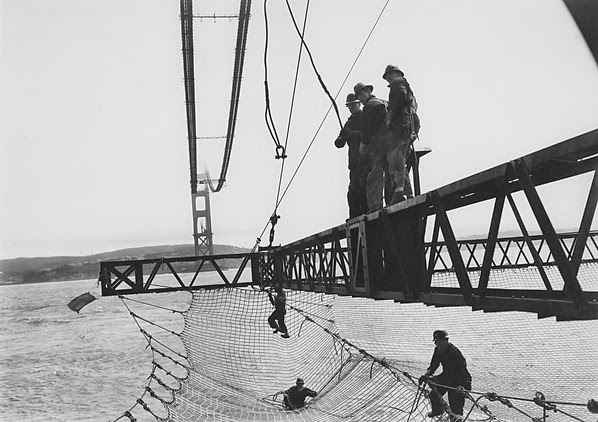
\includegraphics[height=0.65\textheight]{images/safety_net_golden_gate_bridge.jpg}}
            \caption{\tiny \url{https://todayinlaborhistory.wordpress.com/2015/01/05/january-5-1933/}}
    \end{figure}

\end{frame}

\begin{frame}[fragile]
\frametitle{What are Version Control Systems?}
    \begin{multicols}{2}
        \begin{itemize}
            \item Saved states are like anchor points in like rock climbing:
                one can fall back a small distance without losing everything
        \end{itemize}
        \begin{figure}
            \centerline{%
                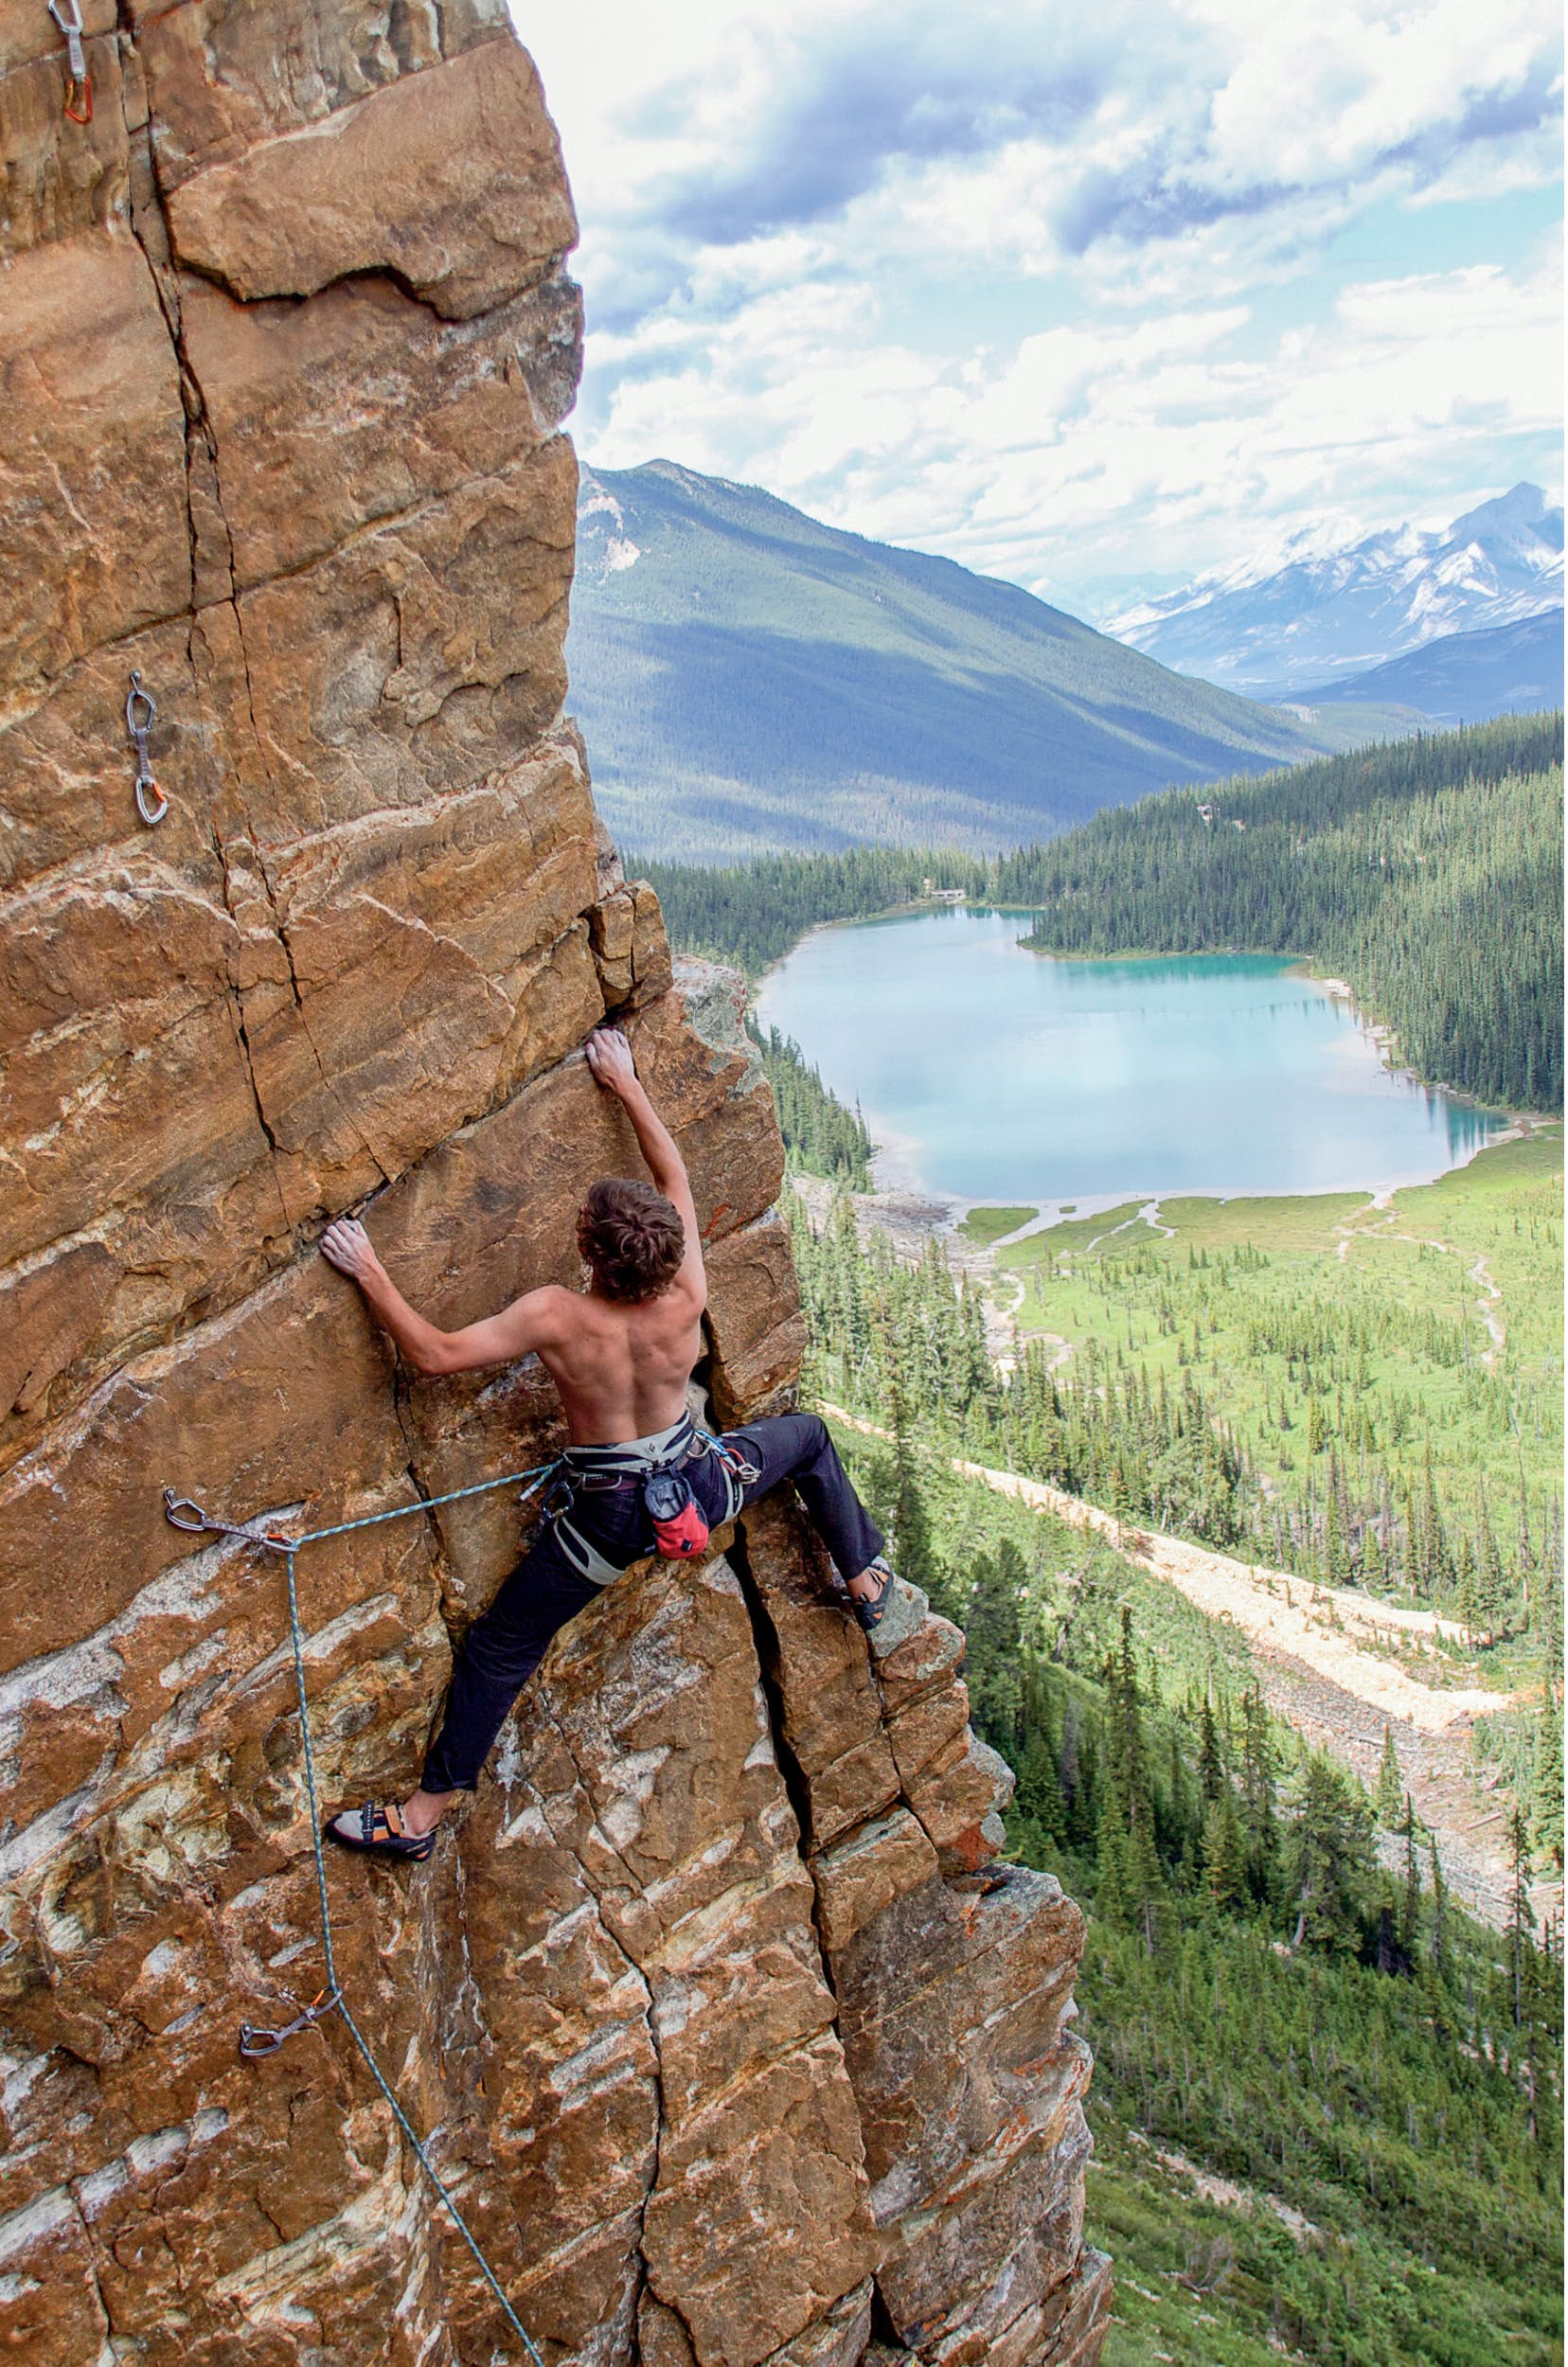
\includegraphics[height=0.8\textheight]{images/northern_exposure_jasper_rock_climbing.jpg}}
                \caption{\tiny by Fran\c{c}ois Laplante, \url{http://www.northernexposurejasper.com/}}
        \end{figure}
    \end{multicols}
\end{frame}

\begin{frame}[fragile]
\frametitle{Why use a Version Control System?}

Does this look familiar?

\begin{lstlisting}
$ ls
file.1      file.20090803  file.keep
file.2      file.alt       file.old
file.old.2  file.fixed     file.new
\end{lstlisting}
%stopzone

This is better than nothing, however \ldots
\begin{itemize}
    \item what happened between the different versions?  And just as
        important: \emph{why}?
    \item which file is actually the most current?
    \item what if \ttt{file.old} is the \emph{newest} file?
    \item can the differences between files tell us anything?
    \item why store \emph{nine} files when we really only need one?
\end{itemize}
\end{frame}

\begin{frame}
\frametitle{Why use a Version Control System?}
\begin{itemize}
    \item Version Control Systems help to tame this chaos
    \item Useful in detecting when bugs were introduced or fixed
    \item Used to save known states of a group of files and hence versions
        (releases) of a software project
    \item Can aid work on collaborative projects
\end{itemize}
\end{frame}

\begin{frame}
\frametitle{Who uses version control?}
\begin{itemize}
    \item Anyone wanting access to an old version of a document.
    \item Anyone working on a collaborative project.
    \item Anyone to whom such things have happened:
        \begin{itemize}
            \item ``It would be nice to have the version from 2 hours ago \ldots''
            \item ``I wrote that really well three days ago.  How did that
                go again?''
            \item ``Oh no!  I deleted the file!''
            \item ``Hrm, the application stopped working.  What changed in the
                last update?''
        \end{itemize}
\end{itemize}
\end{frame}

\begin{frame}
\frametitle{Where is version control used?}
    \begin{itemize}
    \item Software development
    \item Text and document processing/writing
        \begin{itemize}
            \item e.g. books, scientific articles, talks
        \end{itemize}
    \item Graphic and web design
    \item System administration
        \begin{itemize}
            \item track changes to configuration files
            \item the tool \code{etckeeper} automates this process
        \end{itemize}
    \end{itemize}
\end{frame}

\begin{frame}
\frametitle{What should be kept under version control?}
\begin{itemize}
    \item Any kind of file that will be changed
    \item Mainly text files
        \begin{itemize}
        \item Program code, documentation
        \item Theses, dissertations
        \item Configuration files
        \end{itemize}
    \item Binary files also possible
        \begin{itemize}
        \item Graphics files: \code{.png}, \code{.tiff}
        \item Documents: \code{.odt}
        \end{itemize}
\end{itemize}
\end{frame}

\begin{frame}
\frametitle{What \emph{shouldn't} be kept under version control?}
\begin{itemize}
    \item Automatically generated files
        \begin{itemize}
            \item e.g.: \code{.o}, \code{.log}, \code{.pdf}, \code{.pyc}
        \end{itemize}
    \item Editor backup files
        \begin{itemize}
            \item e.g.: \code{file\~{}}, \code{file.bak}
        \end{itemize}
    \item Data files
        \begin{itemize}
            \item e.g. simulation input or output files
            \item are often static or change very seldom
            \item better kept on an FTP server or similar
        \end{itemize}
    \item Large files
        \begin{itemize}
            \item can make cloning a repository very slow
            \item cause unnecessary bloat in repository
        \end{itemize}
\end{itemize}
\end{frame}

\begin{frame}
\frametitle{A short Git History}
\begin{itemize}
    \item Linux kernel development could use proprietary BitKeeper system
        free of charge
    \item The owners of BitKeeper changed the licensing conditions, which
        meant that it was no longer free for kernel developers to use
    \item Thus Linus Torvalds wrote his own system: Git
    \item Open source with a large developer community and an even larger
        user base.
\end{itemize}
\end{frame}

\begin{frame}
    \frametitle{Why use Git?}
    \begin{itemize}
        \item Supports distributed development
        \item Doesn't rely on network availability
        \item Scales to thousands of developers and millions of commits
        \item Fast!
        \item Repositories contain complete project history
        \item Lightweight branches
        \item Atomic operations
        \item Open source
        \item Free as in freedom
    \end{itemize}
\end{frame}

% vim: expandtab shiftwidth=4 softtabstop=4

\section{Installing Git}

\begin{frame}
\frametitle{Installing Git (GUI options)}
There are many GUI clients to choose from.  Here is a selection:
\begin{itemize}
    \item SourceTree
        
\includegraphics[height=0.05\textheight]{images/Sourcetree-blue.pdf}
        \begin{itemize}
            \item \url{https://www.sourcetreeapp.com/}
            \item License: free as in beer
        \end{itemize}
    \item TortoiseGit
        
\includegraphics[height=0.05\textheight]{images/tgit_logo.pdf}
        \begin{itemize}
            \item \url{https://tortoisegit.org/}
            \item License: free as in freedom
        \end{itemize}
    \item Git Extensions
        
\includegraphics[height=0.05\textheight]{images/git-extensions-logo.pdf}
        \begin{itemize}
            \item \url{https://gitextensions.github.io/}
            \item License: free as in freedom
        \end{itemize}
    \item GitKraken
        
\includegraphics[height=0.05\textheight]{images/gitkraken-logo-dark-hz.png}
        \begin{itemize}
            \item \url{https://www.gitkraken.com/}
            \item License: free for non-commercial use
        \end{itemize}
    \item More GUI clients can be found on the Git website:
        \begin{itemize}
            \item \url{https://git-scm.com/download/gui/windows}
        \end{itemize}
\end{itemize}
\end{frame}


\begin{frame}
\frametitle{Use the command line!}
\begin{itemize}
    \item With the command line one can get futher and do more; the
        learning curve is steeper, but it's worth it.
    \item Hence, we will focus on the command line interface (CLI) from now
        on.
\end{itemize}
    \blockquote[Hunt and Thomas, \emph{The Pragmatic Programmer}]
    {Gain familiarity with the shell, and you'll find your productivity soaring.}
\end{frame}


\begin{frame}
\frametitle{Installing Git (CLI options; Windows)}
\begin{itemize}
    \item download the installer from \url{https://git-scm.com/download/win}
    \item double click the downloaded \code{.exe} file and follow the
        installation instructions to install it
\end{itemize}
\end{frame}


\begin{frame}
\frametitle{Installing Git (CLI options; MacOS)}
\begin{itemize}
    \item download the installer from \url{https://git-scm.com/download/mac}
    \item double click the downloaded image file to install it
        % TODO: add installation screens to slides
\end{itemize}
\end{frame}


\begin{frame}[fragile]
\frametitle{Installing Git (CLI options; Linux/Unix)}
\begin{itemize}
    \item either via a package manager, e.g.:
\end{itemize}

\begin{lstlisting}
sudo apt install git  # Debian-based distributions
sudo yum install git  # RedHat-based distributions
\end{lstlisting}

\begin{itemize}
    \item or via the source code:
\end{itemize}

\begin{lstlisting}[
    breaklines=true,
    postbreak=\mbox{$\hookrightarrow$\space}]
wget https://mirrors.edge.kernel.org/pub/software/scm/git/git-<version>.tar.gz
tar -xvzf git-<version>.tar.gz
cd git-<version>
./configure
make
make test  # optional
sudo make install
\end{lstlisting}

\begin{itemize}
    \item more help is available on the Git Linux/Unix download page:
        \url{https://git-scm.com/download/linux}
\end{itemize}
\end{frame}

% vim: expandtab shiftwidth=4:

%%%%%%%%%%%%%%%%%%%%%%%%%%%%%%%%%%%%%%%%%%%%%%%%%%%%%%%%%%%%%%%%%%%%%%%%%%%%

\section{Text editors}

\begin{frame}
\frametitle{Text editors}
\begin{itemize}
    \item We will be creating and editing text files, hence the need for a
        text editor.
    \item One of the fundamental tools of software development.
    \item There are many options to choose from:
    \begin{itemize}
        \item \href{https://notepad-plus-plus.org/}{Notepad++}
        \item \href{https://www.vim.org/}{Vim}, \href{https://www.gnu.org/software/emacs/}{Emacs}
        \item \href{https://atom.io/}{Atom}
        \item \href{https://www.sublimetext.com/}{Sublime text}
        \item \href{https://wiki.gnome.org/Apps/Gedit}{gedit},
            \href{https://kate-editor.org/}{kate}
    \end{itemize}
    \item The choice of editor is unimportant; what \emph{is} important is
        that you feel comfortable using yours.
\end{itemize}
\end{frame}

\section{Initial Git configuration}

\begin{frame}[fragile]
    \frametitle{Detour: setting name and email metadata}
    If this is the first time you've installed Git, then one of the first
    things you need to do is to set your name and email address
    configuration metadata:
\begin{lstlisting}[language=bash]
git config --global user.name "Your name"
git config --global user.email "<username@example.com>"
\end{lstlisting}
\end{frame}

\begin{frame}[fragile]
    \frametitle{Exercise: explore \code{git config}}

    Open a terminal (or the Git-Bash shell in Windows) and enter the
    following commands:
\begin{lstlisting}
git config
git config --list
git config --help
\end{lstlisting}

    \begin{itemize}
        \item describe the output of each command
        \item how does the output relate to the commands mentioned on the
            previous slide?
        \item if you need to find out detailed information about a command,
            what might you always be able to do?
    \end{itemize}
\end{frame}

%%%%%%%%%%%%%%%%%%%%%%%%%%%%%%%%%%%%%%%%%%%%%%%%%%%%%%%%%%%%%%%%%%%%%%%%%%%%
\section{Using Git on your own}

\begin{frame}
\frametitle{Using Git on your own}
\begin{itemize}
    \item Why would one want to use Git alone?
    \item Obtain benefits of version control
        \begin{itemize}
            \item have a safety net
            \item access to a time machine
            \item get a log of changes and why
            \item you are actually another person in six months when you're
                looking back over your work trying to figure out what you've
                done
        \end{itemize}
    \item Can use Git on your own computer
        \begin{itemize}
            \item simple setup and management
            \item no servers to administer
            \item no cloud service necessary
        \end{itemize}
    \item There are even more benefits when working with others; we'll
        discuss this in more detail later in the course
\end{itemize}
\end{frame}


\begin{frame}
    \frametitle{Starting a new repository}
    Steps to create a Git repository:
    \begin{itemize}
        \item create a directory
        \item change into that directory
        \item run \code{git init}
        \item that's it!
    \end{itemize}
\end{frame}


\begin{frame}[fragile]
\frametitle{Exercise: create a new repository}
\begin{itemize}
    \item Create a directory and change into it
\end{itemize}
\begin{lstlisting}
mkdir blupp
cd blupp
\end{lstlisting}
\begin{itemize}
    \item Initialise the repository
\end{itemize}
\begin{lstlisting}
git init
\end{lstlisting}
\begin{itemize}
    \item What's the output of the \code{git init} command?  How does this
        help us?
    \item Explore the directory, what's in there?
    \item Use \code{ls -la} to find the hidden directory.
    \item Run \code{git status} for more info from git.  What's this
        output it telling us?
\end{itemize}
\end{frame}


\begin{frame}[fragile]
\begin{lstlisting}[basicstyle=\tiny\ttfamily]
$ mkdir blupp
$ cd blupp/
$ git init
Initialized empty Git repository in /home/cochrane/blupp/.git/
$ ls
$ ls -ltra
total 28
drwxr-xr-x 117 cochrane cochrane 20480 Nov 21 02:39 ..
drwxr-xr-x   3 cochrane cochrane  4096 Nov 21 02:39 .
drwxr-xr-x   7 cochrane cochrane  4096 Nov 21 02:39 .git
$ ls .git/
branches  config  description  HEAD  hooks  info  objects  refs
$ ls .git/*
.git/config  .git/description  .git/HEAD

.git/branches:

.git/hooks:
applypatch-msg.sample  pre-applypatch.sample      pre-push.sample     update.sample
commit-msg.sample      pre-commit.sample          pre-rebase.sample
post-update.sample     prepare-commit-msg.sample  pre-receive.sample

.git/info:
exclude

.git/objects:
info  pack

.git/refs:
heads  tags
\end{lstlisting}
%stopzone
\end{frame}

\begin{frame}[fragile]
\frametitle{What does git init do?}
\begin{itemize}
    \item Creates a \code{.git} directory
    \item Creates various configuration files, e.g. \code{.git/config}
    \item Sets up the repository; the repository is inside the \code{.git}
        directory
\end{itemize}
\end{frame}

\begin{frame}[fragile]
\begin{lstlisting}[basicstyle=\tiny\ttfamily]
$ git status
On branch master

Initial commit

nothing to commit (create/copy files and use "git add" to track)
\end{lstlisting}
\end{frame}
%stopzone


\begin{frame}[fragile]
\frametitle{Adding files or changes to the repository}
\begin{itemize}
    \item To add files (or changes to files) to the repository's
        staging area, we use the \code{git add} command.
    \begin{itemize}
        \item the \emph{staging area} is where changes to the repository
            are kept before they are committed.
    \end{itemize}
    \item Git now knows to \emph{track} the file for future changes.
    \item \emph{Staging}, \emph{tracking}, and \emph{adding} are all
        roughly equivalent terms for the same process.
\end{itemize}

Let's add a file in tiny steps to see the process in detail:
\begin{lstlisting}
touch moo     # create a file
git status    # check repo status (file is *untracked*)
git add moo   # add file to the staging area
git status    # file is now a change to be committed
\end{lstlisting}
\end{frame}


\begin{frame}[fragile]
\frametitle{Committing files or changes to the repository}
\begin{itemize}
    \item Committing files or changes saves the staged changes into the
        repository.
    \item A commit is a snapshot of the current repository state.
\end{itemize}
\begin{lstlisting}
git status    # file is now a change to be committed
git commit    # commit staged changes to repository
... enter commit message ...
... see brief commit information ...
git status    # working directory now clean
\end{lstlisting}
\end{frame}


\begin{frame}
\frametitle{Add/commit cycle}
The add/commit cycle is like how a photographer creates a group photo.
\end{frame}


\begin{frame}
\frametitle{Starting a new repository from scratch}
\begin{itemize}
    \item mkdir something
    \item cd something
    \item git init  (also ls -la)
    \item git status
    \item create file
    \item git status (untracked)
    \item git add
    \item git status (staged)
    \item git commit
    \item git status (clean)
    \item master is default branch
    \item (normally don't have to run git status all the time)
\end{itemize}
\end{frame}

\begin{frame}
    \frametitle{Starting a new repository (conceptual steps)}
    \begin{itemize}
        \item Create directory for repository (mkdir)
        \item Initialise repository (git init)
        \item Create file(s) (edit file)
        \item Add file(s) to repository (git add)
        \item Commit file(s) (git commit)
    \end{itemize}
\end{frame}

\begin{frame}
\frametitle{Starting a new repository (conceptual steps)}
\begin{itemize}
    \item To create a repository, need to \ttt{init}ialise it
        \begin{itemize}
            \item \code{git init}
        \end{itemize}
    \item Repository is just a directory, with a \code{.git} directory
        \begin{itemize}
            \item \code{ls -la}
        \end{itemize}
    \item Things that go into a repository are just files
        \begin{itemize}
            \item \code{touch file}
        \end{itemize}
    \item To tell Git to track a file, one needs to \ttt{add} it
        \begin{itemize}
            \item \code{git add}
        \end{itemize}
    \item Tracked files and \emph{changes to tracked files} are put in
        the \emph{staging area}
        \begin{itemize}
            \item \code{git status} (see staged files)
        \end{itemize}
    \item To record files and \emph{changes to files}, one \ttt{commit}s
        them to the repository
        \begin{itemize}
            \item \code{git commit}
        \end{itemize}
\end{itemize}
\end{frame}

\begin{frame}
\frametitle{Exercise: Start a new repository}
\begin{itemize}
    \item Repeat the previous steps on your own computer
    \item Create a directory and change into it
    \item Initialise the repository
    \item Run git status to see the current repository state
    \item Create a file (untracked); see the repository state, what changed?
    \item Add the file to the repository (track it); see the repository
        state, what changed?
    \item Commit the file to the repository; see the repository state, what
        changed?
\end{itemize}
\end{frame}

\begin{frame}
\frametitle{Minor detour: Git configuration}
\begin{itemize}
    \item Brief intro to git config
    \item Repo-local config
    \item Global config
\end{itemize}
\end{frame}

\begin{frame}
\frametitle{Getting Help}
\begin{itemize}
    \item man pages
    \item git help
    \item books
    \begin{itemize}
        \item How Git Works; Julia Evans; \url{https://wizardzines.com/zines/git/}
    \end{itemize}
    \item online references
    \begin{itemize}
        \item Git book: \url{https://git-scm.com/doc}
        \item Cheat sheet: \url{https://github.com/dasesu/git/blob/main/Git_quick_reference.pdf}
    \end{itemize}
\end{itemize}
\end{frame}

\begin{frame}
\frametitle{Exercise: git help}
\begin{itemize}
    \item Use \code{git help} on \code{init}, \code{add}, \code{commit} and
        \code{config} commands
    \item Open and browse on \url{https://git-scm.org}
\end{itemize}
\end{frame}

\begin{frame}[fragile]
\frametitle{Parts of a local Git repository}
\begin{columns}[T]
    \begin{column}{0.5\textwidth}
        \begin{itemize}
            \item Working directory
            \item Staging area
            \item Repository
            \item Very important for understanding operations
        \end{itemize}
    \end{column}

    \begin{column}{0.5\textwidth}
        \begin{center}
            \resizebox{!}{0.7\textheight}{
                \documentclass{standalone}
\usepackage{tikz}
\usetikzlibrary{positioning}
\usetikzlibrary{calc}

\begin{document}

\begin{tikzpicture}[
workingdir/.style={circle,
                fill=blue!20!white,
                draw=blue!50!black,
                minimum size=5mm},
staging/.style={circle,
                fill=blue!20!white,
                draw=blue!50!black,
                minimum size=5mm},
repo/.style={circle,
                fill=blue!20!white,
                draw=blue!50!black,
                minimum size=5mm},
link/.style={-, >=stealth, thick}]

% box to represent .git dir
% git add, git commit text
% git commit <file>; git commit -a


\node (working dir) at (0, 0) [workingdir] {working directory};
\node (staging) [staging, above=of working dir] {staging};
\draw [link, <->] (working dir) -- (staging);
\node (repo) [repo, above=of staging] {repository};
\draw [link, <->] (staging) -- (repo);

\draw [link, <->, dashed] (working dir.north east)
    .. controls ($ (staging.east) + (1, 0) $) .. (repo.south east);

\end{tikzpicture}
\end{document}

            }
        \end{center}
    \end{column}
\end{columns}
\end{frame}

\begin{frame}
\frametitle{Snapshots and diffs}
\begin{itemize}
    \item Photograph analogy
    \item Commits build on one another
    \item Working directory: checked out version of local repository
    \item Staging area: what will be committed next
    \item Repository: storage of snapshots
    \item Contrast with other systems, which store diffs between changes
\end{itemize}
\end{frame}

\begin{frame}
\frametitle{Basic workflow}
\begin{itemize}
    \item creation (mkdir, init, edit)
    \item saving snapshots of work (add, commit, return to edit step)
\end{itemize}
\end{frame}

\begin{frame}
\frametitle{Workflow}

Preparation:
\begin{itemize}
    \item \code{git init} (only once)
    \item \code{git checkout}
    \item \code{git config}
\end{itemize}

Main steps:
\begin{itemize}
    \item \code{git add} (before committing a file)
    \item \code{git mv}
    \item \code{git status}
    \item \code{git diff}
    \item \code{git rm}
    \item \code{git log}
    \item \code{git show}
    \item \code{git commit}
\end{itemize}
\end{frame}

\begin{frame}
\frametitle{Specifying commits}
\begin{description}
    \item[\code{c82a22c39c}] SHA hash
    \item[\code{HEAD}] name of the commit
    \item[\code{HEAD\^}] parent of \code{HEAD}
    \item[\code{HEAD\^\^}] grandparent of \code{HEAD}
    \item[\code{HEAD~2}] also grandparent of \code{HEAD}
    \item[\code{HEAD~4}] great-great grandparent of \code{HEAD}
\end{description}

also works with branch names:
\begin{description}
    \item[\code{main\^}] parent of tip of “\code{main}” branch
    \item[\code{main~4}] great-great grandparent of tip of “\code{main}” branch
        experimental tip of “\code{experimental}” branch
\end{description}
\end{frame}

\begin{frame}
\frametitle{Detour: Commit advice}

when, what, how to commit

commit messages

commit a single, focussed idea/concept

small commits have small diffs and are easier for others to review

Recommendations for commits:

\begin{itemize}
    \item A commit should contain a single, self contained idea.
    \item The commit message should contain a short description
        of the idea or change being made in this commit.
    \item A one line subject line
    \item An optional text describing more details of the change. The
        why of the change is important. Remember: this is a
        communication exercise.
    \item Commits should be as small as possible (atomic commits).
\end{itemize}

    http://sethrobertson.github.io/GitBestPractices

How often should I commit?
\begin{itemize}
    \item as often as possible
    \item “release early, release often”
    \item as soon as the changes belonging to a given idea are
        finished
    \item don’t be afraid to commit!
\end{itemize}

\end{frame}

\begin{frame}
\frametitle{Commit advice (cont.)}

\begin{itemize}
    \item Each commit needs a “commit message” describing the
    change
    \item Commit messages document what was done in each
    change and why
    \item An important part of communication within a project:
    \begin{itemize}
        \item commit logs are messages to other people
        \item ... and are messages to yourself in the future!
    \end{itemize}
\end{itemize}

What should I write in a commit message?
\begin{itemize}
    \item a short description of the change
    \item the description can sometimes be longer than the actual
    change! The message describes the “why” of the change.
    \item the message should be able to explain later what
    happened in the change
    \item note: when problems occur, this is where one looks first for
        information
\end{itemize}

\end{frame}

\begin{frame}
\frametitle{Extending the sample project}
\begin{itemize}
    \item edit, add, commit
    \item seeing what we've done
    \begin{itemize}
        \item git log (--graph)
        \item git show
        \item git diff
    \end{itemize}
    \item deleting/renaming files
    \begin{itemize}
        \item git rm
        \item git mv
    \end{itemize}
\end{itemize}
\end{frame}

\begin{frame}
\frametitle{Explain SHAs}
\begin{itemize}
    \item in context of diff, show, log, etc.
\end{itemize}
\end{frame}

\begin{frame}
\frametitle{Exercise: extend the sample project further}
\begin{itemize}
    \item recommended steps \ldots
    \item practice git add/commit/rm/mv
    \item practice git log/show/diff
\end{itemize}
\end{frame}

\begin{frame}
\frametitle{Ignoring files}

To ignore files in Git one simply needs a \code{.gitignore} file with
entries for the files one wishes to ignore. It is possible to use
regular expressions and wildcards such as \code{*.o} in order to ignore
multiple files.

TODO: insert example of creating files to ignore and then creating a
.gitignore file.
\end{frame}

\begin{frame}[fragile]
\frametitle{Ignoring files (cont.)}

Because the \code{.gitignore} file can change (and it’s highly likely
that we’re interested in these changes) one also keeps this file under
version control. We therefore add the file to the repository and commit
it:

\begin{lstlisting}
$ git add .gitignore
$ git commit .gitignore
Created commit 38d2e3c: Ignoring the hallo program
1 files changed, 2 insertions (+) , 0 deletions (-)
create mode 100644 .gitignore
\end{lstlisting}
\end{frame}

\begin{frame}[fragile]
\frametitle{Showing branches}
\code{git show-branch}

\begin{itemize}
    \item shows the available branches
    \item shows with an asterisk \code{*} which is the current branch
\end{itemize}

\begin{lstlisting}
$ git show-branch -- list
* [ master ] Ignoring the hallo program and * ~files
$ git show-branch --more=35
[ master ] Ignoring the hallo program and * ~files
[ master\^ ] Added a southern ’hallo’ variant
[ master~2 ] Initial import of the hallo project
\end{lstlisting}
\end{frame}

\begin{frame}[fragile]
\frametitle{Showing branches (cont.)}
\code{git branch} shows available branches and which branch is
current.

\begin{lstlisting}
$ git branch
* master
\end{lstlisting}

\code{git branch -v} shows the commit hash and the commit
message of the most recent commit.

TODO need more expansive examples here with multiple branches.

\begin{lstlisting}
$ git branch -v
* master 38d2e3c Ignoring the hallo program and *~
\end{lstlisting}
\end{frame}

\begin{frame}
\frametitle{Import existing project}
\begin{itemize}
    \item git init, git add, git commit
\end{itemize}
\end{frame}

\begin{frame}
\frametitle{Aliasing commands}
\begin{itemize}
    \item reduce typing, use alias
    \item handy aliases: st, di, ci, co
\end{itemize}
\end{frame}

\begin{frame}
\frametitle{Staging and unstaging files}
\begin{itemize}
    \item staging area in more depth
    \item unstage files one doesn't want to track
    \item git reset (just moves pointer/label)
\end{itemize}
\end{frame}

\begin{frame}
\frametitle{Exercise!}
\end{frame}

%%%%%%%%%%%%%%%%%%%%%%%%%%%%%%%%%%%%%%%%%%%%%%%%%%%%%%%%%%%%%%%%%%%%%%%%%%%%
\section{Using Git with others}

\begin{frame}
\frametitle{Working with others}
\begin{itemize}
    \item a networked world
    \item version control becomes more interesting when one works with
        others
    \item author and committer can be different people (usually aren't)
    \item work more often with branches (very powerful feature)
\end{itemize}
\end{frame}

\begin{frame}
\frametitle{Working with others (also online)}

\begin{description}
    \item[\code{git clone}] Clones a pre-existing repository; basically copy
        into a new directory and get the current branch
    \item[\code{git pull}] Pull changes from another repo into the local repo
    \item[\code{git push}] Push changes from a local repo into another
    \item[\code{git format-patch}] Generate a patch file, which one can
        then send as an email attachment
\end{description}
\end{frame}

\begin{frame}
\frametitle{Tagging commits}
\end{frame}

\begin{frame}
\frametitle{Add remote repos to model}
\begin{itemize}
    \item working directory
    \item staging area
    \item local repo
    \item remote repo(s)
\end{itemize}
\end{frame}

\begin{frame}
\frametitle{Cloning an existing repo}
\begin{itemize}
    \item git clone
    \item changes to git config --list
    \item explain meaning of origin
    \item master, origin/master, HEAD
\end{itemize}
\end{frame}

\begin{frame}
\frametitle{Exercise!}
\end{frame}

\begin{frame}
\frametitle{Dealing with conflicts}
\begin{itemize}
    \item can happen when working on same part of a file
    \item happens when working with others
    \item happens when working with branches and stashes (hence can also
        happen when one is working alone!)
\end{itemize}
\end{frame}

\begin{frame}
\frametitle{Exercise!}
\end{frame}

\begin{frame}
\frametitle{Branches}
\begin{itemize}
    \item what are they?
    \item why use them?
    \item localise work on a focussed topic
    \item don't interfere with main development on master
    \item allows devs to work on parts of projects independently
    \item allows for code reviews before merging
\end{itemize}
\end{frame}

\begin{frame}
\frametitle{The default branch: master}

Discuss push/pull just from master?  Then have push/pull concept ready
for quick fix example below
\end{frame}

\begin{frame}
\frametitle{Branches}
\begin{itemize}
    \item git branch
    \item git branch -a
    \item git branch <branchname>
    \item git checkout <branchname>
    \item git checkout -b <branchname>
    \item naming branches -> clarity very helpful
\end{itemize}
\end{frame}

\begin{frame}
\frametitle{Simple branch}
\begin{center}
    \resizebox{!}{0.7\textheight}{
        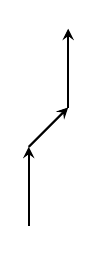
\begin{tikzpicture}
    [link/.style={->, >=stealth, thick}]

\draw [link] (0, 0) -- (0, 1);  % master
\draw [link] (0, 1) -- (0.5, 1.5);
\draw [link] (0.5, 1.5) -- (0.5, 2.5);  % branch

\end{tikzpicture}

    }
\end{center}
\end{frame}

\begin{frame}
\frametitle{Examples and exercises!}
\end{frame}

\begin{frame}
\frametitle{Merging branches}
\begin{itemize}
    \item merge changes on one branch into another
    \item git merge <branchname>
    \item fast-forward merge
    \item merge commits
    \item conflicts can occur (merge conflicts)
\end{itemize}
\end{frame}

\begin{frame}
\frametitle{Merging branches}
\begin{center}
    \resizebox{!}{0.7\textheight}{
        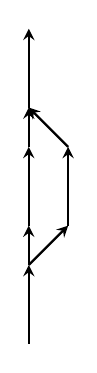
\begin{tikzpicture}
    [link/.style={->, >=stealth, thick}]

\draw [link] (0, 0) -- (0, 1);  % master
\draw [link] (0, 1) -- (0.5, 1.5);
\draw [link] (0.5, 1.5) -- (0.5, 2.5);  % branch
\draw [link] (0.5, 2.5) -- (0, 3);  % merge commit
\draw [link] (0, 3) -- (0, 4);

\draw [link] (0, 1) -- (0, 1.5);
\draw [link] (0, 1.5) -- (0, 2.5);
\draw [link] (0, 2.5) -- (0, 3);

\end{tikzpicture}

    }
\end{center}
\end{frame}

\begin{frame}
\frametitle{Example: quick fix}
\begin{itemize}
    \item when working on a new feature (on a feature branch)
    \item bug found on main branch -> quick fix necessary
    \item commit changes on current branch
    \item checkout master
    \item checkout quick fix branch (git checkout -b <branchname>)
    \item make fix, test, commit
    \item merge into master, push
    \item return to work on feature branch
\end{itemize}
\end{frame}

\begin{frame}
\frametitle{Example: handling merge conflicts}
\begin{itemize}
    \item work on same area of code
    \item try to merge
    \item handle (resolve) conflict
    \item git add (to mark as resolved)
    \item git commit (as necessary)
\end{itemize}
\end{frame}

\begin{frame}
\frametitle{Cherry picking}
\begin{itemize}
    \item associated with merging
    \item only when some commits are wanted
    \item git cherry-pick <commit>
\end{itemize}
\end{frame}

\begin{frame}
\frametitle{Local and remote branches}
\end{frame}

\begin{frame}
\frametitle{Fetching from remotes}
\begin{itemize}
    \item git pull $\approx$ git fetch; git merge
    \item why fetch then merge?
    \item origin is writable but upstream isn't -> common OSS model
    \item define upstream
    \item changes are made on upstream
    \item fetch changes to local repo
    \item merge changes into local branch (e.g. master)
\end{itemize}
\end{frame}

\begin{frame}
\frametitle{Exercise!}
\end{frame}

\begin{frame}
\frametitle{Rewriting history}
\begin{itemize}
    \item unpublished (not yet pushed) changes can be rearranged
    \item reorder, edit, squash, reword, delete (split also possible,
        but more involved)
    \item the story on wants to tell about the development; not all
        commits need to be pushed
    \item allows one to polish the changes; improve quality
    \item linearise changes; published repo has clear, linear history
        (see e.g. Ovid's slide about git histories)
\end{itemize}
\end{frame}

\begin{frame}
\frametitle{Interactive rebase}
\begin{itemize}
    \item git rebase -i
    \item very handy to clean up history before pushing
\end{itemize}
\end{frame}

\begin{frame}
\frametitle{Stashing changes}
\begin{itemize}
    \item why use this?
    \item what is this?
    \item handy feature for interrupted work
    \item e.g. quick fix example
    \item git stash
    \item git stash show -p
    \item git stash pop (conflicts possible)
    \item git stash drop
    \item git stash drop/show {n}
\end{itemize}
\end{frame}

\begin{frame}
\frametitle{Stashing changes}
\code{git stash}
\begin{itemize}
    \item One is in the middle of a task
    \item Something unrelated needs to be fixed quickly
    \item Use \code{git stash} to save the current state (or more
        explicitly: \code{git stash save}
    \item The working copy is now "clean"
    \item One is now able to work on the new topic and check in the
        changes
    \item \code{git stash pop} reinstates the old state
    \item Now one can work on the previous task again, where one
        left off
    \item \code{git stash} works like a stack (push/pop operations)
\end{itemize}
\end{frame}

\begin{frame}
\frametitle{Stashing changes}

\begin{description}
    \item \code{git stash list} List all “stashed” states
    \item \code{git stash show} Show a stashed state
    \item \code{git stash apply} Apply a state to the current working copy
    \item \code{git stash pop} Pop the “top most” state off the stack and
        apply it onto the current working copy
\end{description}
\end{frame}

%%%%%%%%%%%%%%%%%%%%%%%%%%%%%%%%%%%%%%%%%%%%%%%%%%%%%%%%%%%%%%%%%%%%%%%%%%%%
\section{Using a version control system service}

\begin{frame}
    \frametitle{Online VCS services}
    \begin{itemize}
        \item GitHub
        \item GitLab
        \item BitBucket
        \item others?
    \end{itemize}
\end{frame}

\begin{frame}
    \frametitle{Forking a repository}

    - create own repository of another project
    - gives ability to contribute to original project via Pull Requests
    (also called Merge Requests)
    - one can push changes to own fork because it belongs to you
    - pushing changes directly to someone else's project isn't possible
    (unless you have commit access, which isn't default situation)
    - commit changes to a non-`main` branch and push to upstream fork ->
    from here can create Pull Request
    - services like GitHub/GitLab detect such pushes and prompt to create a
    Pull Request
    - fork and pull request has become most common open source collaboration
    workflow (mostly due to GitHub)
    diagram:
    |upstream repo; label: "upstream"|  -> fork -> |upstream fork; label: "origin"|
                        fetch v                            push ^ ; clone v
                                                   |local repo|

    - show screenshots of example of forking a repo on GitHub
\end{frame}

\begin{frame}
    \frametitle{Submitting a Pull Request}
    - a Pull Request is a \emph{proposal} for a code change in an upstream
    project repository.  It is merely \emph{one} way to contribute to a
    project; there are other workflows.
    - the first step is to create a fork of the project repository that
    you're contributing to (see Forking a repository)
    - in your local Git repository of the project, create a feature branch
    git checkout -b "feature_branch_name"
    - build your proposed feature in the feature branch
    - push feature branch to \emph{your} upstream forked repository
    - button will (usually) appear which leads to pull request dialog
    - open pull request dialog, add title (describes proposed changes very
    briefly)
    - add details of what was changed and why this is of value, was
    necessary, is a good idea in the pull request text
    - submit pull request
    - maintainer will be notified by e.g. GitHub automatically
    - maintainer might ask for code to be changed, or want things done
    differently. Be gracious! Try to adhere to project's development
    guidelines. Be respectful! Usually maintainers are unpaid and doing such
    projects in their spare time.
\end{frame}

%%%%%%%%%%%%%%%%%%%%%%%%%%%%%%%%%%%%%%%%%%%%%%%%%%%%%%%%%%%%%%%%%%%%%%%%%%%%

\section{Tricks and tips}

\begin{frame}[fragile]
    \frametitle{Splitting commits}
    \tbf{Problem:} you've committed code that you'd rather have in
        separate commits.

    \tbf{Solution:} use an interactive rebase to edit the commit
        to split; ``undo'' the code changes to separate; add
        modifications; amend the current commit.
        Make ``undone'' changes and commit.  Continue
        the interactive rebase.
\begin{lstlisting}
git rebase -i <branch_name>~<num_commits>
# extract changes to separate
git add <changed_files>
git commit --amend
# add separated changes to files
git commit <changed_files>
git rebase --continue
\end{lstlisting}

    \see{https://stackoverflow.com/questions/6217156/break-a-previous-commit-into-multiple-commits}
\end{frame}

\begin{frame}[fragile]
    \frametitle{Restore a deleted file (simple revert)}
    \tbf{Problem:} a file has been deleted in an earlier commit and you wish
    to restore it.

    \tbf{Solution:} If the file was deleted in a commit of its own, then
    just revert and write an appropriate commit message.
\begin{lstlisting}
git revert <commit_sha>
... explain reason for revert in commit message ...
\end{lstlisting}
\end{frame}

\begin{frame}[fragile]
    \frametitle{Restore a deleted file (restore from SHA)}
    \tbf{Problem:} a file has been deleted in an earlier commit and you wish
    to restore it.

    \tbf{Solution:} If the file was deleted as a part of a larger commit, a
    simple revert is not so simple.  Instead, find the last commit affecting
    the file; this is the commit where it was deleted.  Check out the file
    from this commit's parent commit.  The file is now a newly-added file in
    the working directory.
\begin{lstlisting}
git checkout \
    $(git rev-list -n 1 HEAD -- "$file")^ -- "$file"
\end{lstlisting}
%stopzone

This command finds the most recent commit affecting the file:
\begin{lstlisting}
git rev-list -n 1 HEAD -- "$file"
\end{lstlisting}
%stopzone

    \see{https://stackoverflow.com/questions/953481/find-and-restore-a-deleted-file-in-a-git-repository}
\end{frame}

\begin{frame}[fragile]
    \frametitle{Recover a lost or deleted commit}
    \tbf{Problem:} A rebase or reset has made a commit unreachable.

    \tbf{Solution:} Don't panic! Git doesn't immediately delete commits;
    they are still available via their SHA hash, just not available by
    traversing the commit tree.  Use the reflog to show all operations
    (including ``lost'' commits.  Check out the commit into its own branch
    or simply cherry pick to restore.
\begin{lstlisting}
git reflog
... find commit from commit message ...
git checkout -b <commit_sha>
# or
git cherry-pick <commit_sha>
\end{lstlisting}
%stopzone

    \see{https://stackoverflow.com/questions/10099258/how-can-i-recover-a-lost-commit-in-git}
\end{frame}

\begin{frame}[fragile]
    \frametitle{Find commits affecting a given line in a file (blame)}

    \tbf{Problem:} you want to find the commits corresponding to a given
    line a file.

    \tbf{Solution:} use blame with the line number(s) on the file.

E.g. this command will show the blame from line 150 and the following 11 lines.
\begin{lstlisting}
git blame -L150,+11 -- /path/to/file
\end{lstlisting}

    \see{https://stackoverflow.com/questions/8435343/retrieve-the-commit-log-for-a-specific-line-in-a-file}
\end{frame}

\begin{frame}[fragile]
    \frametitle{Find commits affecting a given line in a file (log)}

    \tbf{Problem:} you want to find the commits corresponding to a given
    line a file.

    \tbf{Solution:} use log with the line number(s) on the file.

    E.g. this command will show the log and a patch (or patches) as a unified diff
    output from commits affecting line 155.
\begin{lstlisting}
git log --pretty=short -u -L 155,155:/path/to/file
\end{lstlisting}

    \see{https://stackoverflow.com/questions/8435343/retrieve-the-commit-log-for-a-specific-line-in-a-file}
\end{frame}

\begin{frame}[fragile]
    \frametitle{Find commits affecting a given line in a file (pick-axe)}

    \tbf{Problem:} you want to find the commits corresponding to a given
    line a file.

    \tbf{Solution:} use log -S (pick-axe) with a pattern matching the line
    in the file(s).  One advantage here is that one can also follow commits
    across renames; although in this case only works for single files.

Works for multiple files:
\begin{lstlisting}
git log -S '<pattern_from_line_in_file>' -- /path/to/file
\end{lstlisting}

Follow renames of single file arguments:
\begin{lstlisting}
git log -S '<pattern_from_line_in_file>' \
    --follow -- /path/to/file
\end{lstlisting}

    \see{https://stackoverflow.com/questions/8435343/retrieve-the-commit-log-for-a-specific-line-in-a-file}
\end{frame}


\begin{frame}[fragile]
    \frametitle{Find commits affecting a given line in a file (Glog)}

    \tbf{Problem:} you want to find the commits corresponding to a given
    line a file.

    \tbf{Solution:} use the Glog command from the vim-fugitive plugin.  Note
    this is only for users of the vim editor.

    Load the file and navigate to the line of interest, then enter (in
    command mode)
\begin{lstlisting}
:Glog
\end{lstlisting}

    See: \url{https://stackoverflow.com/a/29261649}
\end{frame}

\begin{frame}[fragile]
    \frametitle{Clean up remote references}

    \tbf{Problem:} \code{git branch -a} shows branches which have been
    deleted in the remote repository.

    This situation can occur if a shared feature branch is deleted by
    someone other than you, or you have a remote feature branch which you
    have deleted via e.g. the ``delete branch'' feature on GitHub's website.
    The local references to the now non-existent remote branches still exist
    and just need to be brought up to date with the current remote state.

    \tbf{Solution:} Use the \code{prune} option to \code{git remote}.

\begin{lstlisting}
git remote prune <remote_alias>
# e.g.:
git remote prune origin
\end{lstlisting}
\end{frame}

\begin{frame}[fragile]
    \frametitle{Find out current branch}
    \begin{lstlisting}
    git branch  // starred branch is current branch
    git branch -a  // starred branch is current branch
    git branch --show-current  // returns name of current branch
    git symbolic-ref --short HEAD  // returns name of current branch (after Git version 1.8)
    git rev-parse --abbrev-ref HEAD  // returns name of current branch (before Git version 2.22)
    \end{lstlisting}
    \href{https://stackoverflow.com/questions/6245570/how-to-get-the-current-branch-name-in-git}{How to get the current branch name in Git?}
\end{frame}

\begin{frame}[fragile]
    \frametitle{Find out where current branch diverged from upstream master}
    \begin{lstlisting}
    git merge-base --fork-point origin/master <branch-name>
    \end{lstlisting}
\end{frame}

\begin{frame}[fragile]
    \frametitle{Run test suite on all commits in given range}
    \begin{lstlisting}
    git rebase -i <branch_name>~x -x '<test command>'
    \end{lstlisting}
\end{frame}

\begin{frame}[fragile]
    \frametitle{Find diff between most recent stash and current working dir}
    \begin{lstlisting}
    git stash show -l
    \end{lstlisting}

    This shows the diff between the current working directory and the most
    recent stash. Not documented in the \ttt{git stash} man page (for version
    2.20.1), but good to know.

    Solution spotted here: https://stackoverflow.com/a/54534613/10874800
\end{frame}

\begin{frame}[fragile]
    \frametitle{Update local submodules from the upstream repo}

    \begin{lstlisting}
    git submodule update --remote --merge
    \end{lstlisting}
\end{frame}

\begin{frame}[fragile]
    \frametitle{Update submodule URL}

    ... which can happen if one moves the submodule's repo to a different
    location.

    \begin{lstlisting}
    # update the submodule url
    git config --file=.gitmodules submodule.<submodule-name>.url <new-repo-url>
    # synchronise the submodule
    git submodule sync
    # update the submodule from the upstream repo
    git submodule update --init --recursive --remote
    \end{lstlisting}

    Some hints gleaned from here:
    https://dev.to/serhatteker/changing-git-submodule-repository-to-other-url-branch-356p

    Check that the tip commit of the updated submodule is the tip commit
    that you expect (i.e. check the submodule's repo and compare its tip
    commit with where the submodule is used).
\end{frame}

\begin{frame}
\frametitle{Extras}
git-worktree - Manage multiple working trees
\end{frame}

\section{Further reading}

\begin{frame}
\frametitle{Further reading}
\begin{itemize}
    \item \href{http://jwiegley.github.io/git-from-the-bottom-up/}{Git from the Bottom Up}
    \item \href{http://tbaggery.com/2008/04/19/a-note-about-git-commit-messages.html}
               {A note about commit messages}
    \item \href{https://xdg.me/blog/a-survey-of-git-best-practices/}
               {A survey of git best practices}
    \item \href{http://kamalmarhubi.com/blog/2016/03/08/git-rebase-exec-make-sure-your-tests-pass-at-each-commit-and-other-rebase-goodies/}
               {git rebase --exec: make sure your tests pass at each commit!  (and other rebase goodies)}
    \item \href{https://ohshitgit.com/}{Oh Shit, Git!?!  Help for getting out of a mess.}
    \item \href{https://jwiegley.github.io/git-from-the-bottom-up/}{Git from the bottom up}
    \item \href{https://cbea.ms/git-commit/}{How to write a git commit message}
\end{itemize}
\end{frame}

\begin{frame}
    \frametitle{Extras}
    \begin{itemize}
        \item Graphically display commits and branches in the terminal
        \item \texttt{git log --graph --oneline --decorate --all}
        \item Visualizing Git Concepts with D3
        \item \url{https://onlywei.github.io/explain-git-with-d3/}
    \end{itemize}
\end{frame}

\section{Deleting a remote branch}

\begin{frame}[fragile]
    \frametitle{Deleting a remote branch once you are finished with it}

\begin{lstlisting}
# as of git 1.7.0
git push origin --delete <branch-name>
# previously
git push origin :<branch-name>
\end{lstlisting}
\end{frame}

\section{Deleting a remote tag}

\begin{frame}[fragile]
\frametitle{Deleting a remote tag}

\begin{lstlisting}
# as of git 1.7.0
git push --delete origin tagname
# previously
git push origin :tagname
\end{lstlisting}

Delete a local tag via \texttt{git tag}:
\begin{lstlisting}
git tag -d tagname
\end{lstlisting}
\end{frame}

\begin{frame}[fragile]
\frametitle{Checking branch merge status}
    \begin{lstlisting}
    git branch --merged master lists branches merged into master

    git branch --merged lists branches merged into HEAD (i.e. tip of current
    branch)

    git branch --no-merged lists branches that have not been merged

    By default this applies to only the local branches. The -a flag will
    show both local and remote branches, and the -r flag shows only the
    remote branches.
    \end{lstlisting}
    source: https://stackoverflow.com/a/227026/10874800
\end{frame}

\begin{frame}[fragile]
\frametitle{Setting the executable bit on Windows Git}
Windows will show files as being executable, but the executable bit won't be
set when adding and committing files in Git Bash.  Here's a workaround:
    \begin{lstlisting}
    find . -name '*.sh' | xargs git update-index --chmod=+x
    \end{lstlisting}
    source: https://stackoverflow.com/a/32717779/10874800
\end{frame}

\begin{frame}[fragile]
\frametitle{Extract single commit as patch}
\begin{lstlisting}
git format-patch -1 f8aae4
\end{lstlisting}
\end{frame}

\begin{frame}[fragile]
\frametitle{Extracting subdir into separate repo}
used to have to use git filter branch:
    https://stackoverflow.com/a/359759/10874800

    new-repo-name: name of the new repository, derived from subdir of
    old-repo-name

For example:
    \begin{lstlisting}
git clone git@<server-name>:<orig-repo-name>.git <new-repo-name>
cd <new-repo-name>/
# delete all commits that don't have anything to do with the `orders` directory
git filter-branch --prune-empty --subdirectory-filter orders master
git remote set-url origin git@<server-name>:<new-repo-name>.git
# fix incorrect email addresses in commits
git filter-branch --original refs/correct_email_orig --env-filter '
OLD_EMAIL="paul@<old-email-provider>"
CORRECT_NAME="Paul Cochrane"
CORRECT_EMAIL="paul.cochrane@<new-email-provider>"
if [ "$GIT_COMMITTER_EMAIL" = "$OLD_EMAIL" ]
then
export GIT_COMMITTER_NAME="$CORRECT_NAME"
export GIT_COMMITTER_EMAIL="$CORRECT_EMAIL"
fi
if [ "$GIT_AUTHOR_EMAIL" = "$OLD_EMAIL" ]
then
export GIT_AUTHOR_NAME="$CORRECT_NAME"
export GIT_AUTHOR_EMAIL="$CORRECT_EMAIL"
fi
' --tag-name-filter cat -- --branches --tags
git push -u origin master
    \end{lstlisting}

but now can use git subtree:
    https://stackoverflow.com/a/17864475/10874800

\begin{lstlisting}
cd <old-repo-name>
git subtree split -P <subdir-name>/ -b <new-repo-name>
cd ..
mkdir <new-repo-name>
cd <new-repo-name>/
git init
git pull ../<old-repo-name>/ <new-repo-name>
git remote add origin git@<server-name>:<new-repo-name>.git
git push origin -u master
cd ../<old-repo-name>/
git rm -rf <subdir-name>/
git ci
git push
git branch -D <subdir-name>  # <= TODO check that this step is correct!
\end{lstlisting}
\end{frame}

\appendix

\section{Version Control System models}

\begin{frame}
    \frametitle{Version Control System models}
    \begin{itemize}
        \item Local
        \item Centralised
        \item Distributed
    \end{itemize}
\end{frame}

\begin{frame}
\frametitle{Local Model}
        % -> image/diagram of local system
\begin{itemize}
    \item Restricted to a single computer
    \item Historically also only able to be used by one person at a time
        (e.g. access control via file locking)
    \item Examples:
        \begin{itemize}
            \item \href{https://en.wikipedia.org/wiki/Revision_Control_System}
                       {Revision Control System (RCS)}
            \item \href{https://en.wikipedia.org/wiki/Source_Code_Control_System}
                       {Source Code Control System (SCCS)}
        \end{itemize}
\end{itemize}
\end{frame}

\begin{frame}[fragile]
\frametitle{Centralised Model}
\begin{columns}[T]
    \begin{column}{0.7\textwidth}
        \begin{itemize}
            \item Client-Server architecture
            \item Server contains all repository files and is ``single source of truth''
            \item Clients contain copies of repository, where one work on project
                files (\emph{working copy})
            \item Require network access to server for version control actions
            \item Examples:
            \begin{itemize}
                \item \href{https://en.wikipedia.org/wiki/Concurrent_Versions_System}
                           {Concurrent Versions System (CVS)}
                \item \href{https://en.wikipedia.org/wiki/Apache_Subversion}
                           {Subversion (SVN)}
            \end{itemize}
        \end{itemize}
    \end{column}
    \begin{column}{0.4\textwidth}
        \begin{center}
        \resizebox{\textwidth}{!}{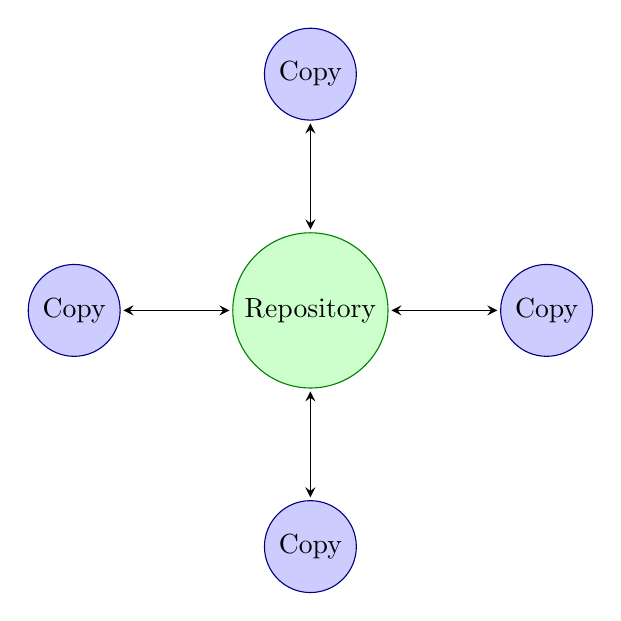
\begin{tikzpicture}
[repo/.style={circle,
		fill=green!20!white,
		draw=green!50!black,
		minimum size=10mm},
workingcopy/.style={circle,
		fill=blue!20!white,
		draw=blue!50!black,
		minimum size=5mm},
link/.style={<->, shorten <=1pt, shorten >=1pt, >=stealth, semithick}]

% central repo
\node at (0, 0) [repo] (mainrepo) { Repository };
% working copies
\node at (3,0)  [workingcopy] (copyright)  { Copy };
\node at (-3,0) [workingcopy] (copyleft)   { Copy };
\node at (0,3)  [workingcopy] (copytop)    { Copy };
\node at (0,-3) [workingcopy] (copybottom) { Copy };
% links between repo and working copies
\draw [link] (mainrepo) -- (copyright);
\draw [link] (mainrepo) -- (copyleft);
\draw [link] (mainrepo) -- (copytop);
\draw [link] (mainrepo) -- (copybottom);
\end{tikzpicture}
}
        \end{center}
    \end{column}
\end{columns}
\end{frame}

\begin{frame}
\frametitle{Distributed Model}
        % -> image/diagram of distributed system
\begin{itemize}
    \item Client-Server or Peer-to-peer or a mixture of the two
    \item Each client has complete repository and its entire history
    \item Server no longer strictly required; if used, contains a ``bare''
        version of the repository, i.e. the working directory is not present
    \item Offline work now possible and simple
    \item When collaborating can resync work when online again
    \item Examples:
        \begin{itemize}
            \item \href{https://git-scm.com/}{Git}
                
\includegraphics[height=0.05\textheight]{images/git_logo.png}
            \item \href{https://www.mercurial-scm.org/}{Mercurial}
                
\includegraphics[height=0.05\textheight]{images/mercurial_logo.png}
        \end{itemize}
\end{itemize}
\end{frame}


\begin{frame}
\frametitle{Leftover notes from old git/svn course}
merging commits: git rebase -i <commit>

splitting commits: git rebase -i <commit> - mark which commit
to edit - when rebase reaches that commit use

git reset HEAD\^ to reset before the commit but keep your
working tree intact - incrementally add changes and commit
them (git add -p can be useful) - run git rebase –continue to
proceed applying the commits after the now-split commit
(adapted from
http://stackoverflow.com/questions/4307095/git-how-to-split-up-a-commit-buried-in-history)

reordering commits: git rebase -i <commit>
pick, squash, edit

http://www.gitready.com/advanced/2009/02/10/squashing-commits-with-rebase.html

http://www.gitready.com/advanced/2009/03/20/reorder-commits-with-rebase.html

git config --global color.ui auto -> automatically colour diffs,
logs and other git output

git diff --word-diff -> do a diff on words and not on lines. Per
default in colour, but if don’t have a colour terminal minus
signs (-) and plus signs (+) are used around words to show
what has been removed or added respectively.

create bare repo -> clone -> make commits in local repo -> git
push -> error -> why? A: because there isn’t a branch on the
server, there needs to be a connection between the local

”master” branch and the ”origin” on the server, hence one
needs to run ”git push origin master” in order to make this
connection.
\end{frame}


% good git helper talk
% C'mon git happy; John Anderson; PerlCon Pittsburgh 2019
% https://youtu.be/oEKXV-_o3YQ


\begin{frame}{Merge git repositories into one}

solution found here: https://medium.com/altcampus/how-to-merge-two-or-multiple-git-repositories-into-one-9f8a5209913f
# enter the working directory of an existing repo to merge into
cd Bewerbungen/
# add other repo as remote and fetch its commits
git remote add --fetch job-apps git@bitbucket.org:paultcochrane/job_applications.git
# merge new repo into repo of pwd
# note --allow-unrelated-histories to allow merge to work
# otherwise error
git merge job-apps/master --allow-unrelated-histories
# remove now unnecessary remote
git remote remove job-apps

\end{frame}

\end{document}

\begin{frame}{Interactive rebasing with root commit}
    Usually the root commit is excluded from a rebase.  However, sometimes
    it's necessary to edit this commit as well as any others following.  For
    example, let's say the first 4 commits have been created.  We later find
    changes which should have been part of the initial (root) commit (e.g. we
    missed adding a file), then it would be necessary to change the root
    commit.  To do this we can use the --root option to rebase:

    git rebase -i --root

    which then runs an interactive rebase but also showing the root commit.
    Then it's possible to add the missing changes to the root commit, say by
    creating a commit adding those changes and then squashing this extra
    commit into the initial (root) commit.

    See also:
    https://mariusschulz.com/blog/how-to-squash-the-first-two-commits-in-a-git-repository
\end{frame}

% vim: expandtab shiftwidth=4:
